\documentclass{article}
\usepackage{amsmath,amssymb}
\usepackage{enumitem}
\usepackage{graphicx}

\begin{document}

\begin{center}
\Large\textbf{CM1025 Fundamentals of Computer Science}\\
\large\textbf{Midterm Assessment}\\
\vspace{0.5cm}
\large\textbf{Student Number: 250151349}\\
\large\textbf{Name: Ryo Nakayama}\\
\vspace{1cm}
\end{center}

\section*{Question 1}

\subsection*{(a)}

\textbf{Determine whether the following are logically equivalent:}

\[
(P \lor Q) \rightarrow R \quad \text{and} \quad (P \rightarrow R) \land (Q \rightarrow R)
\]

We prove both directions logically:

\begin{itemize}
  \item[$\Rightarrow$] Assume \((P \lor Q) \rightarrow R\) is true.  
  If \(P\) is true, then \(P \lor Q\) is true, so \(R\) must be true. Thus, \(P \rightarrow R\).  
  Likewise, if \(Q\) is true, then \(P \lor Q\) is true, so again \(R\) must be true. Thus, \(Q \rightarrow R\).  
  Therefore, \((P \rightarrow R) \land (Q \rightarrow R)\) holds.

  \item[$\Leftarrow$] Assume \((P \rightarrow R) \land (Q \rightarrow R)\) is true.  
  Then, if \(P \lor Q\) is true, at least one of \(P\) or \(Q\) is true.  
  In either case, \(R\) must be true.  
  Therefore, \((P \lor Q) \rightarrow R\) holds.
\end{itemize}

\subsection*{(b)}

\textbf{Which of the following is a tautology?}

\begin{itemize}
  \item A. \(P \lor \neg P\): Always true (Law of the excluded middle). ✅
  \item B. \(P \land \neg P\): Always false (Contradiction). ❌
  \item C. \(P \leftrightarrow P\): Always true (Identity). ✅
  \item D. \(P \rightarrow P\): Always true (Implication to itself). ✅
\end{itemize}

\textbf{Answer:} The tautologies are A, C, and D.  
Therefore, the correct choice is not E.  
\textbf{Correct answer: A, C, and D}

\subsection*{(c)}

\textbf{Prove that } \(P \rightarrow (Q \rightarrow R)\) \textbf{ is logically equivalent to } \((P \land Q) \rightarrow R\) \textbf{ using logical equivalences only.}

\begin{align*}
P \rightarrow (Q \rightarrow R)
&\equiv \neg P \lor (Q \rightarrow R) && \text{(Implication)} \\
&\equiv \neg P \lor (\neg Q \lor R) && \text{(Implication)} \\
&\equiv (\neg P \lor \neg Q) \lor R && \text{(Associativity)}
\end{align*}

Now for the right-hand side:

\begin{align*}
(P \land Q) \rightarrow R
&\equiv \neg (P \land Q) \lor R && \text{(Implication)} \\
&\equiv (\neg P \lor \neg Q) \lor R && \text{(De Morgan)}
\end{align*}

\textbf{Conclusion:} Both expressions reduce to the same form.  
Therefore, they are logically equivalent.

\subsection*{(d)}

\textbf{Translate the statement into formal logic and determine if the structure is valid.}

Let the predicates be:

\begin{itemize}
  \item \(C(x)\): "x owns a cat"
  \item \(L(x)\): "x loves animals"
\end{itemize}

The statements become:

\begin{align*}
&\text{Premise 1: } \forall x (C(x) \rightarrow L(x)) \\
&\text{Premise 2: } \exists x \, C(x) \\
&\text{Conclusion: } \therefore \exists x \, L(x)
\end{align*}

\textbf{Validity:}  
From \(\exists x \, C(x)\), we know that some person, say \(a\), owns a cat.  
By \(\forall x (C(x) \rightarrow L(x))\), we get \(C(a) \rightarrow L(a)\), so \(L(a)\) holds.  
Thus, \(\exists x \, L(x)\) follows.  

\textbf{Conclusion:} The argument is valid.

\section*{Question 2}

\subsection*{(a)}

\textbf{Claim:} If \(f : \mathbb{R} \to \mathbb{R}\) is continuous and \(f(x) \ne 0\) for all \(x \in \mathbb{R}\), then \(\frac{1}{f(x)}\) is also continuous.

\textbf{Proof by contrapositive:}

Assume \(\frac{1}{f(x)}\) is not continuous.  
Then, by properties of reciprocal functions, this can only happen if \(f(x)\) approaches 0 or equals 0 at some point.  
That is, \(f(x) = 0\) or gets arbitrarily close to 0.  
But this contradicts the assumption that \(f(x) \ne 0\) for all \(x\).  

Therefore, the contrapositive is false, which means the original statement is true.  
\(\frac{1}{f(x)}\) must be continuous.

\textbf{Conclusion:} \(\frac{1}{f(x)}\) is continuous under the given conditions.

\subsection*{(b)}

\textbf{Claim:} If \(\sqrt{2} \cdot \sqrt{3}\) is rational, then both \(\sqrt{2}\) and \(\sqrt{3}\) must be rational.

\textbf{Proof:}  
Assume \(\sqrt{2} \cdot \sqrt{3}\) is rational, and suppose at least one of \(\sqrt{2}\) or \(\sqrt{3}\) is irrational.  
Without loss of generality, suppose \(\sqrt{2}\) is irrational.  
Then we write:

\[
\sqrt{3} = \frac{\sqrt{2} \cdot \sqrt{3}}{\sqrt{2}}
\]

Since \(\sqrt{2} \cdot \sqrt{3}\) is rational (by assumption), and \(\sqrt{2}\) is irrational, the quotient should be irrational.  
But we get \(\sqrt{3}\), which must be rational under this expression.  
Contradiction.

\textbf{Conclusion:} If the product is rational, then neither factor can be irrational.  
Thus, both \(\sqrt{2}\) and \(\sqrt{3}\) must be rational.

\subsection*{(c)}

\textbf{Count the number of non-negative integer solutions to:}

\[
x + y + z = 12 \quad \text{subject to } x \leq 5,\ y \leq 6,\ z \leq 7
\]

We fix \(x\) from 0 to 5. For each value of \(x\), we fix \(y\) such that \(y \leq 6\) and \(z = 12 - x - y\) satisfies \(0 \leq z \leq 7\). We count how many such combinations exist.

\begin{itemize}
  \item \(x = 0\): 4 values
  \item \(x = 1\): 5 values
  \item \(x = 2\): 6 values
  \item \(x = 3\): 7 values
  \item \(x = 4\): 6 values
  \item \(x = 5\): 5 values
\end{itemize}

\[
\text{Total solutions} = 4 + 5 + 6 + 7 + 6 + 5 = \boxed{28}
\]

\subsection*{(d)}

\textbf{Count the number of circular arrangements of 6 people where two specific people are not adjacent.}

\textbf{Step 1:} Total circular arrangements:
\[
(6 - 1)! = 120
\]

\textbf{Step 2:} Treat the pair as a block:
\[
(5 - 1)! \times 2 = 24 \times 2 = 48
\]

\textbf{Step 3:} Subtract:
\[
120 - 48 = \boxed{72}
\]

\textbf{Answer:} \fbox{72}

\section*{Question 3}

\subsection*{(a)}

\textbf{How many people must be in a room to guarantee that at least two people share a birthday, assuming 365 possible birthdays (ignoring leap years)? Use the Pigeonhole Principle to answer this question.}

\textbf{Solution:}  
By the Pigeonhole Principle, if there are more people than available birthdays, at least two people must share a birthday.  
There are 365 possible birthdays.  
Therefore, if we have 366 people, by assigning each person to a birthday "box", at least one box must contain two or more people.

\textbf{Answer:} \fbox{366}

\subsection*{(b)}

\textbf{How many 8-character passwords can be made using only lowercase English letters, such that:}

\begin{enumerate}[label=\roman*.]
  \item Each password contains at least one vowel.
  \item No letter repeats.
\end{enumerate}

There are 26 lowercase letters: 5 vowels and 21 consonants.  
We want all 8-letter permutations using distinct letters that include \textbf{at least one vowel}.

\textbf{Step 1: Total permutations with no repeated letters:}

\[
P(26, 8) = 26 \times 25 \times \cdots \times 19
\]

\textbf{Step 2: Subtract permutations that use only consonants (no vowels):}

\[
P(21, 8) = 21 \times 20 \times \cdots \times 14
\]

\textbf{Answer:}

\[
\boxed{P(26, 8) - P(21, 8)}
\]

\subsection*{(c)}

\textbf{How many integer solutions are there to the equation:}

\[
x_1 + x_2 + x_3 + x_4 = 20
\]

\textbf{Subject to:}
\begin{itemize}
  \item \(x_i > 1\)
  \item \(x_i \ne 2, 3\)
\end{itemize}

\textbf{Step 1: Determine allowed values for each \(x_i\)}

Since \(x_i > 1\), and \(x_i \ne 2,3\), the smallest possible value is 4.  
Therefore, each variable must be in the set:
\[
\{4,5,6,\dots\}
\]
We now want all 4-tuples \((x_1,x_2,x_3,x_4)\) such that:
\[
x_1 + x_2 + x_3 + x_4 = 20 \quad \text{and} \quad x_i \in \{4,5,6,\dots\}
\]

\textbf{Step 2: Enumerate all valid compositions (unordered)}

We manually list all unordered 4-tuples summing to 20 with each value \(\geq 4\), skipping 2 and 3:

\begin{itemize}
  \item (4, 4, 4, 8)
  \item (4, 4, 5, 7)
  \item (4, 4, 6, 6)
  \item (4, 5, 5, 6)
  \item (5, 5, 5, 5)
\end{itemize}

All other permutations are just reorderings of these 5 base compositions.

\textbf{Step 3: Count permutations for each composition}

\begin{itemize}
  \item (4, 4, 4, 8): \(\frac{4!}{3!1!} = 4\)
  \item (4, 4, 5, 7): \(\frac{4!}{2!1!1!} = 12\)
  \item (4, 4, 6, 6): \(\frac{4!}{2!2!} = 6\)
  \item (4, 5, 5, 6): \(\frac{4!}{2!1!1!} = 12\)
  \item (5, 5, 5, 5): \(\frac{4!}{4!} = 1\)
\end{itemize}

\[
\text{Total number of integer solutions} = 4 + 12 + 6 + 12 + 1 = \boxed{35}
\]

\textbf{Conclusion:}  
There are \(\boxed{35}\) integer solutions to the equation under the given constraints.

\section*{Question 4}

\subsection*{(a) i.}

\textbf{Design a deterministic finite automaton (DFA) that accepts all binary strings that contain the substring “101”.}

We construct a DFA that recognizes any binary string containing the substring “101”.  
The DFA keeps track of how much of the pattern "101" has been seen so far.

\begin{itemize}
  \item \(q_0\): Start state — no relevant input seen yet
  \item \(q_1\): Saw a leading '1'
  \item \(q_2\): Saw '10'
  \item \(q_3\): Saw '101' — accepting state
\end{itemize}

The transition function is defined as:

\[
\begin{aligned}
&\delta(q_0, 0) = q_0,\quad \delta(q_0, 1) = q_1 \\
&\delta(q_1, 0) = q_2,\quad \delta(q_1, 1) = q_1 \\
&\delta(q_2, 0) = q_0,\quad \delta(q_2, 1) = q_3 \\
&\delta(q_3, 0) = q_3,\quad \delta(q_3, 1) = q_3
\end{aligned}
\]

The diagram of this DFA is shown below:

\begin{center}
  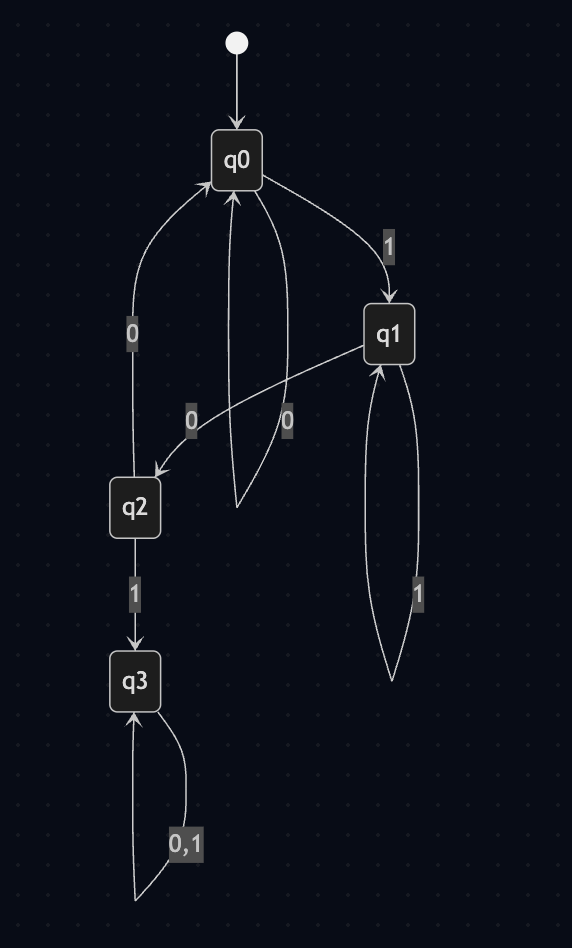
\includegraphics[width=0.5\textwidth]{q4-a-i.png}
\end{center}

\textbf{Accepting state:} \(q_3\)  
\textbf{Start state:} \(q_0\)

This DFA accepts all binary strings that contain the substring "101".

\subsection*{(a) ii.}

\textbf{Find a string that causes the automaton to enter a loop and then exit that loop to reach an accepting state. What is the minimal (shortest length) such string?}

We analyze the DFA constructed for substring "101":

\begin{itemize}
  \item From \(q_0\), input '1' takes the automaton to \(q_1\)
  \item At \(q_1\), reading additional '1' keeps it in a loop: \(\delta(q_1, 1) = q_1\)
  \item To exit the loop: input '0' moves to \(q_2\), then '1' reaches accepting state \(q_3\)
\end{itemize}

\textbf{Therefore, the shortest string that enters a loop and exits it to reach acceptance is:}
\[
\boxed{\texttt{1101}}
\]

This string:
\begin{itemize}
  \item Loops in \(q_1\) on the second '1'
  \item Then follows the transition \(q_1 \xrightarrow{0} q_2 \xrightarrow{1} q_3\)
\end{itemize}

\textbf{Minimal length:} \(\boxed{4}\)

\subsection*{(a) iii.}

\textbf{The automaton accepts strings that contain exactly two 1s. Modify it so that it accepts strings with an even number of 1s. Give an accepted string under the new rules but not under the old.}

\textbf{Modified DFA:}

We define a DFA with two states:
\begin{itemize}
  \item \(q_{even}\): even number of 1s seen (start and accepting state)
  \item \(q_{odd}\): odd number of 1s seen
\end{itemize}

\textbf{Transition function:}
\[
\begin{aligned}
&\delta(q_{even}, 0) = q_{even} \\
&\delta(q_{even}, 1) = q_{odd} \\
&\delta(q_{odd}, 0) = q_{odd} \\
&\delta(q_{odd}, 1) = q_{even}
\end{aligned}
\]

\textbf{Example string:} \texttt{1111}

\begin{itemize}
  \item Contains 4 ones: accepted under the new DFA (even number of 1s)
  \item Rejected under the old DFA, which only accepts strings with exactly 2 ones
\end{itemize}

\textbf{Answer:} \fbox{1111}

\subsection*{(b)}

\textbf{Given a DFA with 5 states over \(\Sigma = \{0,1\}\), it accepts all strings that:}

\begin{itemize}
  \item Do not contain the substring “11”
  \item End in “0”
\end{itemize}

\textbf{Regular expression:}
\[
(0 \mid 10)^*0
\]

\textbf{Plain English description:}

All binary strings that:
\begin{itemize}
  \item contain only 0s and the pattern 10
  \item and end in 0
\end{itemize}

These strings never contain two consecutive 1s.

\section*{Question 5}

\subsection*{(a)}

\textbf{Write a regular expression for passwords with:}
\begin{itemize}
  \item At least one digit
  \item Only letters and digits
  \item No spaces or special characters
\end{itemize}

\textbf{Regular expression:}

\[
\verb!^(?=.*[0-9])[A-Za-z0-9]+$!
\]

\textbf{Explanation:}
\begin{itemize}
  \item \verb!(?=.*[0-9])! ensures that the string contains at least one digit
  \item \verb![A-Za-z0-9]+! allows only letters and digits, one or more times
  \item \verb!^...$! anchors the match to the entire string
\end{itemize}

\subsection*{(b)}

\textbf{Describe a regular language where all strings contain “101” but never contain “111”.}

\textbf{Description:}

The language consists of all binary strings over \(\{0,1\}\) such that:

\begin{itemize}
  \item The substring “101” appears at least once
  \item The substring “111” does not appear anywhere
\end{itemize}

In plain English: all strings must include “101” somewhere in the sequence, but must never include “111”.

This language is regular because both conditions can be enforced using a finite automaton.

\subsection*{(c)}

\textbf{Prove using the Pumping Lemma that the language}

\[
L = \{ a^p \mid p \text{ is a prime number} \}
\]

\textbf{is not regular.}

\textbf{Proof (by contradiction using the Pumping Lemma):}

Assume, for contradiction, that \(L\) is regular.  
Then by the Pumping Lemma, there exists a pumping length \(p \geq 1\) such that every string \(s \in L\) with \(|s| \geq p\) can be written as \(s = xyz\) satisfying:

\begin{itemize}
  \item \(|xy| \leq p\)
  \item \(|y| > 0\)
  \item For all \(i \geq 0\), \(xy^i z \in L\)
\end{itemize}

Choose \(s = a^q \in L\), where \(q\) is a prime number such that \(q \geq p\).  
By the lemma, we can write \(s = xyz\) with \(|xy| \leq p\) and \(|y| > 0\).  
Since \(|xy| \leq p\), the string \(y\) consists only of the letter \(a\) and is entirely within the first \(p\) characters.

Let \(|y| = k > 0\).  
Then, for any \(i \geq 0\), the string \(xy^i z = a^{q + (i-1)k}\)

Now choose \(i = 2\).  
Then the new string is \(a^{q + k}\).  
Since \(k \geq 1\), \(q + k > q\).  
But \(q + k\) is not necessarily prime — we can choose \(q\) and \(k\) such that \(q + k\) is composite.  
Thus, \(xy^2 z \notin L\)

This contradicts the Pumping Lemma.

\textbf{Conclusion:} \(L\) is not regular.

\subsection*{(d)}

\textbf{Provide an example of a string that belongs to the language generated by the context-free grammar G1, but not to the language generated by G2, where G1 and G2 differ in their production rules for recursive structures.}

\textbf{Example:}

Let the grammars be:

\begin{itemize}
  \item G1: \(S \rightarrow S a \mid b\)
  \item G2: \(S \rightarrow a S \mid b\)
\end{itemize}

Then:

\begin{itemize}
  \item \(L(G1) = \{ b, ba, baa, baaa, \dots \}\) — strings that begin with \(b\)
  \item \(L(G2) = \{ b, ab, aab, aaab, \dots \}\) — strings that end with \(b\)
\end{itemize}

\textbf{Therefore, the string \texttt{"ba"} is in \(L(G1)\), but not in \(L(G2)\).}

\[
\textbf{Answer: } \boxed{\texttt{ba}}
\]

\end{document}
